\section{Resultados} \label{sec:resultados}

\subsection{Rotações}

    \begin{figure}[H]
    \centering\hfill
    \begin{subfigure}{0.4\textwidth}
        \centering
        
\includegraphics[width=0.9\textwidth]{rotacoes/16_alp_viz.png}
        \caption{~\texttt{vizinho}.}
    \end{subfigure}%
    \hfill%
    \begin{subfigure}{0.4\textwidth}
        \centering
        
\includegraphics[width=0.9\textwidth]{rotacoes/16_alp_bil.png}
        \caption{~\texttt{bilinear}.}
    \end{subfigure}\hfill
    \\[8pt]\hfill
    \begin{subfigure}{0.4\textwidth}
        \centering
        \includegraphics[width=0.9\textwidth]{rotacoes/16_alp_bic.png}
        \caption{~\texttt{bicubica}.}
    \end{subfigure}%
    \hfill%
    \begin{subfigure}{0.4\textwidth}
        \centering
        \includegraphics[width=0.9\textwidth]{rotacoes/16_alp_lag.png}
        \caption{~\texttt{lagrange}.}
    \end{subfigure}\hfill

    \caption{Rotação de 15\textdegree{} no plano da imagem aplicada em \texttt{house16.png} ($16 \times 16$).}
    \label{fig:house16:alp}
\end{figure}

    Na \cref{fig:rot:house64}, podemos ver com clareza a diferença entre os métodos. Nas interpolações bilinear e bicúbica, a imagem resultante aparece com um pequeno borramento. Esse efeito é bem mais fraco com polinômios de Lagrange.

    Para o aproximação por vizinho mais próximo, a figura fica com um serrilhado bem presente, principalmente nas bordas. Isso aparece inclusive em imagens grandes, como na \cref{fig:rot:house}. Além desse método, quase não existem diferenças visuais para as imagens de $512 \times 512$.

    \begin{figure}[H]
    \centering
    \begin{subfigure}{0.3\textwidth}
        \centering
        \includegraphics[width=0.8\textwidth]{rotacoes/64_alp_viz.png}
        \caption{~\texttt{vizinho}.}
    \end{subfigure}%
    \hspace{8pt}%
    \begin{subfigure}{0.3\textwidth}
        \centering
        \includegraphics[width=0.8\textwidth]{rotacoes/64_alp_bil.png}
        \caption{~\texttt{bilinear}.}
    \end{subfigure}
    \\[8pt]
    \begin{subfigure}{0.3\textwidth}
        \centering
        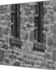
\includegraphics[width=0.8\textwidth]{rotacoes/64_alp_bic.png}
        \caption{~\texttt{bicubica}.}
    \end{subfigure}%
    \hspace{8pt}%
    \begin{subfigure}{0.3\textwidth}
        \centering
        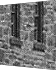
\includegraphics[width=0.8\textwidth]{rotacoes/64_alp_lag.png}
        \caption{~\texttt{lagrange}.}
    \end{subfigure}

    \caption{Rotação de -30\textdegree{} no plano da imagem aplicada em \texttt{house16.png} ($64 \times 64$).}
    \label{fig:rot:house64}
\end{figure}

    \begin{figure}[H]
    \centering
    \begin{subfigure}{0.33\textwidth}
        \centering
        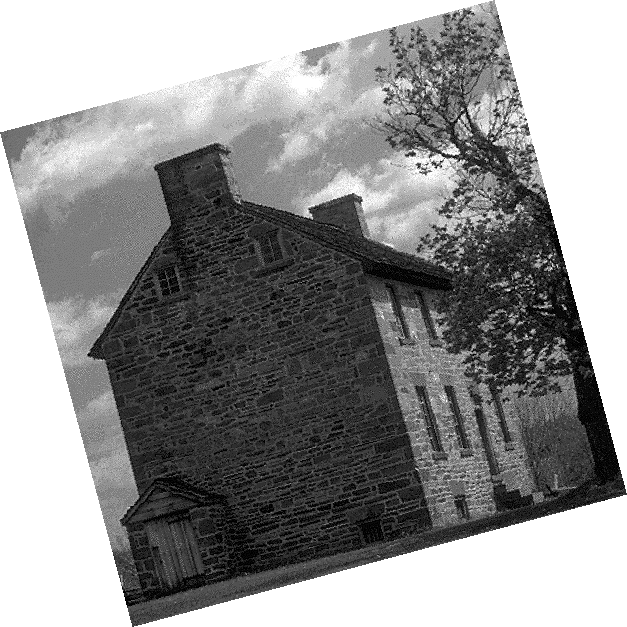
\includegraphics[width=0.9\textwidth]{rotacoes/house_alp_viz.png}
        \caption{~\texttt{vizinho}.}
    \end{subfigure}%
    \hspace{8pt}
    \begin{subfigure}{0.33\textwidth}
        \centering
        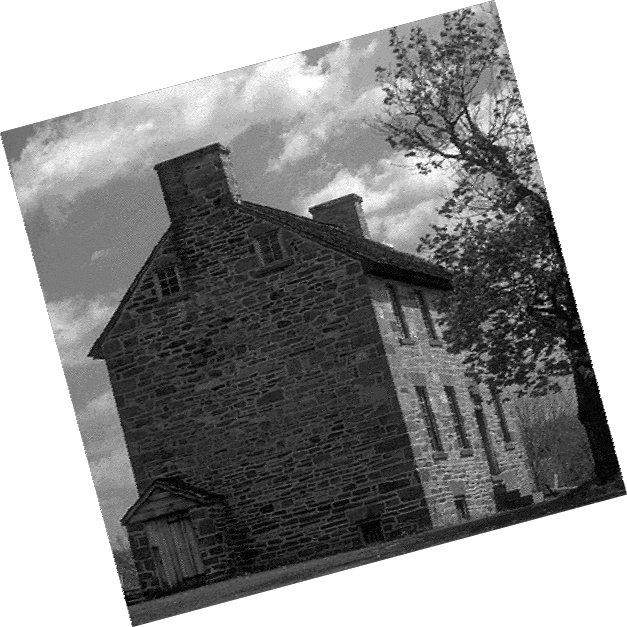
\includegraphics[width=0.9\textwidth]{rotacoes/house_alp_bil.png}
        \caption{~\texttt{bilinear}.}
    \end{subfigure}
    \\[8pt]
    \begin{subfigure}{0.33\textwidth}
        \centering
        \includegraphics[width=0.9\textwidth]{rotacoes/house_alp_bic.png}
        \caption{~\texttt{bicubica}.}
    \end{subfigure}%
    \hspace{8pt}%
    \begin{subfigure}{0.33\textwidth}
        \centering
        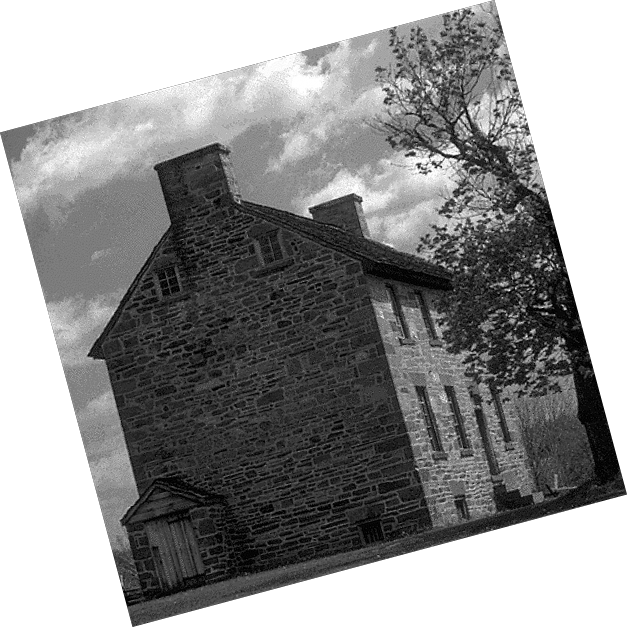
\includegraphics[width=0.9\textwidth]{rotacoes/house_alp_lag.png}
        \caption{~\texttt{lagrange}.}
    \end{subfigure}

    \caption{Rotação de 15\textdegree{} no plano da imagem aplicada em \texttt{house.png} ($512 \times 512$).}
    \label{fig:rot:house}
\end{figure}

\subsection{Escalonamento}

    \begin{figure}[H]
    \centering
    \begin{subfigure}{0.3\textwidth}
        \centering
        \includegraphics[width=0.9\textwidth]{escala/city_13_viz.png}
        \caption{~\texttt{vizinho}.}
    \end{subfigure}%
    \hspace{8pt}
    \begin{subfigure}{0.3\textwidth}
        \centering
        \includegraphics[width=0.9\textwidth]{escala/city_13_bil.png}
        \caption{~\texttt{bilinear}.}
    \end{subfigure}
    \\[8pt]
    \begin{subfigure}{0.3\textwidth}
        \centering
        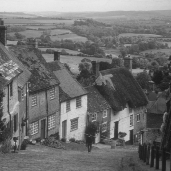
\includegraphics[width=0.9\textwidth]{escala/city_13_bic.png}
        \caption{~\texttt{bicubica}.}
    \end{subfigure}%
    \hspace{8pt}%
    \begin{subfigure}{0.3\textwidth}
        \centering
        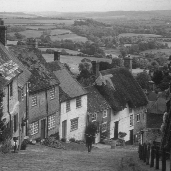
\includegraphics[width=0.9\textwidth]{escala/city_13_lag.png}
        \caption{~\texttt{lagrange}.}
    \end{subfigure}

    \caption{Escalonamento com $S_x = S_y = 1/3$ aplicado em \texttt{city.png} ($512 \times 512$).}
    \label{fig:esc:13}
\end{figure}

    \begin{figure}[H]
    \centering
    \begin{subfigure}{0.3\textwidth}
        \centering
        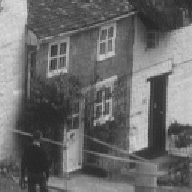
\includegraphics[width=0.9\textwidth]{escala/128_15_viz.png}
        \caption{~\texttt{vizinho}.}
    \end{subfigure}%
    \hspace{8pt}
    \begin{subfigure}{0.3\textwidth}
        \centering
        \includegraphics[width=0.9\textwidth]{escala/128_15_bil.png}
        \caption{~\texttt{bilinear}.}
        \label{fig:esc:15:bil}
    \end{subfigure}
    \\[8pt]
    \begin{subfigure}{0.3\textwidth}
        \centering
        \includegraphics[width=0.9\textwidth]{escala/128_15_bic.png}
        \caption{~\texttt{bicubica}.}
    \end{subfigure}%
    \hspace{8pt}%
    \begin{subfigure}{0.3\textwidth}
        \centering
        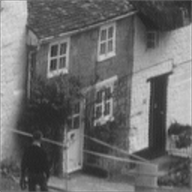
\includegraphics[width=0.9\textwidth]{escala/128_15_lag.png}
        \caption{~\texttt{lagrange}.}
    \end{subfigure}

    \caption{Escalonamento com $S_x = S_y = 1.5$ aplicado em \texttt{city128.png} ($128 \times 128$).}
    \label{fig:esc:15}
\end{figure}

    No caso da mudança de escala, podemos ver que a bicúbica tem os melhores resultados na redução das dimensões, que acontece na \cref{fig:esc:13}. No entanto, para ampliação da imagem (\cref{fig:esc:15}), o borramento da imagem é muito forte, fazendo com que o método por polinômios de Lagrange tenha resultados melhores. Isso também acontece na \cref{fig:esc:86}, por ser muito pequeno o resultado.

    Tanto na ampliação (\ref{fig:esc:15:bil}), quanto na redução (\ref{fig:esc:13:bil}), o método bilinear gerou artefatos muito presentes nas bordas dos objetos. No entanto, isso pode ser devido à implementação e não necessariamente ao método. Um efeito similar aconteceu usando os vizinhos mais próximos.

    \begin{figure}[H]
    \centering
    \begin{subfigure}{0.33\textwidth}
        \centering
        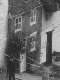
\includegraphics[width=0.8\textwidth]{escala/128_86_viz.png}
        \caption{~\texttt{vizinho}.}
    \end{subfigure}%
    \hspace{8pt}
    \begin{subfigure}{0.33\textwidth}
        \centering
        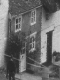
\includegraphics[width=0.8\textwidth]{escala/128_86_bil.png}
        \caption{~\texttt{bilinear}.}
    \end{subfigure}
    \\[8pt]
    \begin{subfigure}{0.33\textwidth}
        \centering
        \includegraphics[width=0.8\textwidth]{escala/128_86_bic.png}
        \caption{~\texttt{bicubica}.}
    \end{subfigure}%
    \hspace{8pt}%
    \begin{subfigure}{0.33\textwidth}
        \centering
        \includegraphics[width=0.8\textwidth]{escala/128_86_lag.png}
        \caption{~\texttt{lagrange}.}
    \end{subfigure}

    \caption{Redimensionamento para $80 \times 60$ aplicado em \texttt{city128.png} ($128 \times 128$).}
    \label{fig:esc:86}
\end{figure}

\subsection{Reconstrução}

    \begin{figure}[H]
        \centering
        \includegraphics[width=0.27\textwidth]{../imagens/baboon128.png}
        \caption{\texttt{baboon128.png} ($128 \times 128$).}
        \label{fig:baboon128}
    \end{figure}

    Tentando aplicar uma transformação simples, de escala (\cref{fig:rec:x2}) ou de rotação (\cref{fig:rec:45}), seguida da sua inversa podemos ver que as interpolações bilinear e bicúbica causam um efeito de \textit{blur} muito presente. Para valores racionais, como $S_x = S_y = 1.37$, pode ser que o arredondamento acabe causando artefatos maiores no método dos vizinhos mais próximos.

    \begin{figure}[H]
    \centering
    \begin{subfigure}{0.3\textwidth}
        \centering
        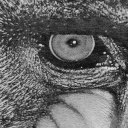
\includegraphics[width=0.9\textwidth]{reconstrucao/baboon_x2_viz.png}
        \caption{~\texttt{vizinho}.}
    \end{subfigure}%
    \hspace{8pt}
    \begin{subfigure}{0.3\textwidth}
        \centering
        \includegraphics[width=0.9\textwidth]{reconstrucao/baboon_x2_bil.png}
        \caption{~\texttt{bilinear}.}
    \end{subfigure}
    \\[8pt]
    \begin{subfigure}{0.3\textwidth}
        \centering
        \includegraphics[width=0.9\textwidth]{reconstrucao/baboon_x2_bic.png}
        \caption{~\texttt{bicubica}.}
    \end{subfigure}%
    \hspace{8pt}%
    \begin{subfigure}{0.3\textwidth}
        \centering
        \includegraphics[width=0.9\textwidth]{reconstrucao/baboon_x2_lag.png}
        \caption{~\texttt{lagrange}.}
    \end{subfigure}

    \caption{Escalonamento por um fator 2 seguido de outro escalonamento de fator 1/2 em \texttt{baboon128.png}, usando o mesmo método em cada caso.}
    \label{fig:rec:x2}
\end{figure}

    \begin{figure}[H]
    \centering
    \begin{subfigure}{0.33\textwidth}
        \centering
        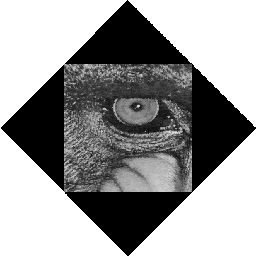
\includegraphics[width=0.95\textwidth]{reconstrucao/baboon_45_viz.png}
        \caption{~\texttt{vizinho}.}
    \end{subfigure}%
    \hspace{8pt}
    \begin{subfigure}{0.33\textwidth}
        \centering
        \includegraphics[width=0.95\textwidth]{reconstrucao/baboon_45_bil.png}
        \caption{~\texttt{bilinear}.}
    \end{subfigure}
    \\[8pt]
    \begin{subfigure}{0.33\textwidth}
        \centering
        \includegraphics[width=0.95\textwidth]{reconstrucao/baboon_45_bic.png}
        \caption{~\texttt{bicubica}.}
    \end{subfigure}%
    \hspace{8pt}%
    \begin{subfigure}{0.33\textwidth}
        \centering
        \includegraphics[width=0.95\textwidth]{reconstrucao/baboon_45_lag.png}
        \caption{~\texttt{lagrange}.}
    \end{subfigure}

    \caption{Rotação de 45\textdegree{} (com borda preta) seguida de outra rotação de -45\textdegree{} no plano da imagem em \texttt{baboon128.png}, usando o mesmo método em cada caso.}
    \label{fig:rec:x2}
\end{figure}

\subsection{Tempo de Execução}

    \begin{figure}[H]
        \centering
        \includegraphics[width=0.3\textwidth]{../imagens/among.png}
        \caption{\texttt{among.png} ($2000 \times 1544$).}
        \label{fig:among}
    \end{figure}

    Para testar a eficiência computacional de cada método, a imagem \texttt{among.png} (\ref{fig:among}) foi rotacionada e escalonada por 2, gerando uma imagem final de dimensões $4867 \times 4112$ pixels em RGBA, ou seja, com 4 canais de cores. O tempo de execução pode ser medido na própria ferramenta, no modo verboso \mintinline{bash}{-v}, como exemplificado abaixo para o método \texttt{lagrange}.

    \begin{minted}[style=vs]{bash}
        $ python3 transforma.py imagens/among.png -o saida.png -v \
            -c r -a 22 -b 20 -e 2 -m lagrange
        INFO:root:imagem imagens/among.png de dimensões (2000, 1544, 4)
        INFO:root:transformação em 0.34468913078308105 segundos
        INFO:root:interpolação em 23.732824563980103 segundos
    \end{minted}

    Cada método também foi executado com um dos \textit{profilers} padrões de Python, o \texttt{cProfile} \autocite{cprofile}. O profiler é capaz de mostrar o tempo de cada função separadamente e cumulativamente. Por exemplo, uma execução do método \texttt{bicubica}, poderia ter o seguinte resultado:

    \begin{minted}[style=vs]{bash}
        $ python3 -m cProfile -s cumtime \
            transforma.py imagens/among.png -o saida.png \
            -c r -a 22 -b 20 -e 2 -m bicubica
            149578 function calls (145313 primitive calls) in 46.493 seconds

            Ordered by: cumulative time

            ncalls  tottime  percall  cumtime  percall filename:lineno(function)
             467/1    0.001    0.000   46.493   46.493 {built-in method builtins.exec}
                 1    0.000    0.000   46.493   46.493 transforma.py:1(<module>)
                 1    0.020    0.020   45.205   45.205 interp.py:23(__call__)
                 1    9.408    9.408   45.185   45.185 interp.py:125(bicubica)
                32    8.006    0.250   23.462    0.733 interp.py:138(R)
               128   15.454    0.121   15.455    0.121 interp.py:130(Pe3)
                16   11.768    0.735   11.768    0.736 idx.py:75(acesso)
                 1    0.000    0.000    0.685    0.685 inout.py:77(imgwrite)
        ...
    \end{minted}

    Os resultados de uma execução estão na \cref{tab:tempo}. Por mais que foi apenas uma execução, outros testes obtiveram resultados similares, oscilando em menos de $20\%$. Como os valores são bem distintos, isso é o bastante para a análise.

    \begin{table}[t]
    \caption{Tempos de execução dos métodos e das funções principais.}
    \label{tab:tempo}

    \centering
    \begin{tabular}{cccccc}
        \toprule\toprule
         & Parte ou Função & \texttt{vizinho} & \texttt{bilinear} & \texttt{bicubica} & \texttt{lagrange} \\
        \midrule
        \multirow{2}{*}{Opção \texttt{-v}}
        & Transformação & 351 ms & 347 ms & 348 ms & 346 ms \\
        & Interpolação & 0.96 s & 4.84 s & 46.27 s & 23.45 s \\
        \midrule
        \multirow{9}{*}{\texttt{cProfile}}
        & \texttt{transforma.py:} & \multirow{2}{*}{0.351 s} & \multirow{2}{*}{0.347 s} & \multirow{2}{*}{0.343 s} & \multirow{2}{*}{0.345 s} \\
        & \texttt{(transformacao)} & & & & \\
        & \texttt{interp.py:(\_\_call\_\_)} & 0.950 s & 4.762 s & 45.963 s & 23.527 s \\
        & \texttt{idx.py:(acesso)}  & 0.801 s & 3.087 s & 12.440 s & 12.062 s \\
        & \texttt{interp.py:(modf)}  & --- & 0.237 s & 0.236 s & 0.238 s \\
        & \texttt{interp.py:(asimg)}  & --- & 0.183 s & 0.305 s & 0.288 s \\
        & \texttt{interp.py:(R)}  & --- & --- & 23.578 s & --- \\
        & \texttt{interp.py:(Pe3)}  & --- & --- & 15.538 s & --- \\
        & \texttt{interp.py:(L)}  & --- & --- & --- & 20.921 s \\
        \bottomrule\bottomrule
    \end{tabular}
\end{table}
